
\documentclass[12pt,twoside]{article}
\usepackage{amssymb, amsmath, mathrsfs, epsfig,amsfonts}
\usepackage{fancyhdr}
\usepackage{microtype}
\setlength{\voffset}{-1in}
\setlength{\topmargin}{0in}
\setlength{\textheight}{9.5in}
\setlength{\textwidth}{6.5in}
\setlength{\hoffset}{0in}
\setlength{\oddsidemargin}{0in}
\setlength{\evensidemargin}{0in}
\setlength{\marginparsep}{0in}
\setlength{\marginparwidth}{0in}
\setlength{\headsep}{0.25in}
\setlength{\headheight}{0.5in}
\pagestyle{fancy}


\fancyhead[LO,LE]{Topological Data Analysis}
\fancyhead[RO,RE]{Tutorial Lab I}
\chead{}
\cfoot{}
\fancyfoot[LO,LE]{}
\fancyfoot[RO,RE]{Page \thepage\ of \pageref{LastPage}}
\renewcommand{\footrulewidth}{0.5pt}
\parindent 0in

\newcommand{\ben}{\begin{enumerate}}
\newcommand{\een}{\end{enumerate}}
\newcommand{\R}{\mathbb{R}}
\newcommand{\Sp}{\vspace{.5in}}
\newcommand{\defn}{\paragraph*{Definition}}
\newcommand{\example}{\paragraph*{Example}}
\newcommand{\examples}{\paragraph*{Examples}}
\newcommand{\qns}{\paragraph*{Questions}}
\newcommand{\qn}{\paragraph*{Question}}
\newcommand{\blank}[1]{\underline{\hspace{#1}}}
\newcommand{\dsst}{\displaystyle}
\newcommand{\fcenter}[1]{\begin{center}\fbox{#1}\end{center}}
\newcommand{\codelist}[1]{\fbox{\scriptsize\texttt{#1}}}


\begin{document}
\begin{center}
{\large\textbf{Harmonics, Morse Filtrations, and 0-Dimensional Persistence}}   
\end{center}

\section{Sampling}

In this section, we will examine the effect of sampling density on the persistence diagram of data sampled from a pure harmonic.  Let's develop some notation to illuminate this:

\defn Let $f^p(x)$ be a pure harmonic of period $p$ (e.g. $f^p(x)=\sin(2\pi x/p )$).  Let $f^p_n$ be sample of $n$ points from $f^p$.  Let $Dgm_0(f^p)$ be the 0-dimensional persistence diagram of $f$, filtered by height.  Note that $p$ can be vector, in which case we get a sum of harmonics.\\

\textbf{Note:} Unless needed, we will drop the $p$ and use $f$ (rather than $f^p$), assuming $p$ is specified.

\subsection{Working it out by Hand}
\label{sect:hand}

\qn Let $p=1$.  \begin{enumerate}

   
   \item Suppose the domain of $f$ is $\mathbb{R}$.  Draw $Dgm_0(f)$ by hand.\vfill
   \item \label{qn:truncint} Now suppose that the domain of $f$ is truncated to a closed interval that includes more than one period (e.g. $[-5,5]$).  Draw $Dgm_0(f)$ by hand.\vfill
   % Note: the next line should be done computationally rather than morally.  Do this after they have compuational tools
   %\item What is $\dsst\lim_{n\to\infty} Dgm_0(f_n)$?\\ \\
\end{enumerate}

\pagebreak

\subsection{Computational Tools}
Now that we know what these objects should look like, it's time to learn computational tools that will allow us to quickly compute and visualize persistence.\\

First, open Matlab and ensure that your environment is correctly set up  by running the following command:

\begin{verbatim}
   >> A=generate_harmonic(-1,1,1000,[1],[1],0);
   >> plot(A(:,1),A(:,2),'.');
\end{verbatim}

If your environment works correctly, you should see a plot of 1,000 points sampled from a harmonic function of period $1$ and amplitude $1$ on the interval $[-1,1]$.  If you get any errors, or if you do not see this, ask your instructor.\\

To generate samples from harmonic functions, use the following utility command:
\begin{center}
\codelist{\texttt{generate\_harmonic(min, max, numsamples, list\_of\_periods, list\_of\_amplitudes, amplitude\_of\_noise)}}
\end{center}
 


where \verb|min| and \verb|max| are the endpoints of the interval, \verb|numsamples| is the number of points to sample.  The rest of the parameters are (hopefully!) self-explanatory.\\

Now, let's generate samples from this harmonic, plot persistence diagrams and see if we can draw conclusions.  We will sample only from the above harmonic (period 1, interval $[-5,5]$).  For now, we will not add any noise.

\begin{enumerate}
   \item Create three objects, $A$, $B$, and $C$.  These should be 10-, 15-, and 25-point samples from the harmonic.
   \item Use the command \verb|morseFiltration(data)| to compute the $0$-dimensional persistence diagram for each of your three samples.  Then use the \verb|plotpersistencediagram(intervals)| to plot them.  (Notes: You should only be passing on $y$-values to the \verb|morseFiltration| command, so use (e.g.) \verb|morseFiltration(A(:,2))|.  The latter command takes the output of the former as input.)
   \item How do the diagrams compare to your answer in Section \ref{sect:hand}, Question \ref{qn:truncint}?\\ \\
   \item Explain your results in a few short sentences.  Specifically, explain what happens to the diagrams as the number of sampled points increases.  You may want to look at the actual intervals you generated, not just the plot.\vfill
\pagebreak
   \item Expand upon your explanation from the previous question in light of the stability theorem for persistence diagrams.\vfill
\end{enumerate}



\section{Making Some Noise}

%\emph{Add noise.  Samples of $<40$ won't show anything new of interest at noise level 0.1, so sample 50, 100, 1000 points at noise level 0.1.  Increase amp of noise and see what happens.  At what point does the signal get swallowed by the noise?}\\

In practice, no data collection method ever gives perfect results.  There is always noise, distorting the samples.  Therefore, understanding how such noise affects persistence diagrams is important.\\

Suppose I take a perfect harmonic (such as the function $f(x)$ from the previous section) and add a bit of bounded noise to it.  I might get the following curve:

\begin{center}
   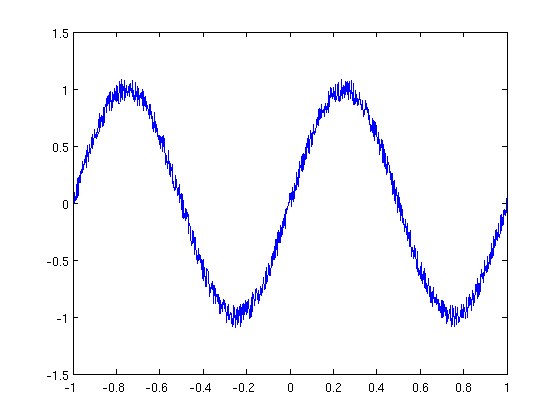
\includegraphics[width=3in]{noisysin}
\end{center}

\qn  Draw (by hand) a possible such diagram for this curve.  Highlight (in a different color) the points that come from the curve, rather than from the added noise.\vfill
\pagebreak

To generate the above curve, I used the following command:
\begin{verbatim}
   >> generate_harmonic(-1,1,1000,[1],[1],0.1);
\end{verbatim}

\qn Explain what this command does.  You may want to refer to the source code for \verb|generate_harmonic|.\vspace{0.5in}

\qn Suppose I increased the amplitude of the noise.  What do you expect will happen to $Dgm_0$?\vfill

\qns Now, we will use our computational tools to investigate the effect of noise, and see if we get what we expect.\begin{enumerate}
   \item For a fixed number of samples (say, $n=100$ points), investigate the effect of adding noise of increasing amplitude $\epsilon$.\vfill\vfill
   \item For a fixed noise amplitude (say, $\epsilon=0.2$), investigate the effect of increasing $n$, the number of points sampled.\vfill\vfill
\end{enumerate}

\pagebreak

\section{Layered Harmonizing}
% Do the same for mixed harmonics, first by hand, then by computer.  Compare, contrast, and explain.

Of course, most signals aren't a pure single harmonic.  As you know from your study of Fourier series, many periodic signals can be decomposed into a weighted sum of harmonics.  (Note: the exact conditions under which a signal has such a decomposition are quite interesting, but not relevant here.)  In this section, we will study the persistence diagrams of mixed harmonic functions.\\

First, consider the mixed harmonic function $f(x)=\sin(2\pi x)+2\sin(\pi x)$.  

\qns \begin{enumerate}   
   \item Suppose the domain of $f$ is $\mathbb{R}$.  Draw $Dgm_0(f)$ by hand.\vfill
   \item Now suppose that the domain of $f$ is truncated to a closed interval that includes more than one period (e.g. $[-5,5]$).  Draw $Dgm_0(f)$ by hand.\vfill
\end{enumerate}

As we did before, we will computationally investigate sampling from this signal and see what happens as our number of samples increases.

\qn Write a \verb|generate_harmonic| command that will sample from $f(x)$ over the interval $[-5,5]$, with no noise added.\vspace{0.5in}

\pagebreak

\qn Use your command above to generate samples with $n=50$, $100$, $500$, and $1,000$ points over the domain $[-5,5]$. Be sure to zoom in around each of the dots in your figures.  Sketch the diagrams here, and explain your results below.  Can you identify which point on the diagrams comes from the truncation?

\pagebreak

\qn Now, generate data from the same harmonic, but on the interval $[-1000,1000]$, still with no noise.  Try sampling $1,250$, $1,500$, $2,000$, $2,500$, $5,000$, $10,000$, $25,000$, and $50,000$ points.  Zoom in on each of the point clusters.  Can you think of a way to decide computationally which cluster comes from the truncation?  What about deciding which artifacts come from undersampling?\vfill


\pagebreak

\qn Returning to a domain of $[-5,5]$, investigate what happens as you add noise to the harmonic and sample a fixed number of points.  It may be worth your time attempting this with a much larger fixed number of samples for a larger domain.  What conclusions can you draw?\vfill

\pagebreak


\section{Noise or Music?}

Run the \verb|loadmasterset| command.  This will create a variable (actually, a cell array) called \emph{masterset}.  The first column of the array consists of 120 data sets, divided into four sets: simple periodic functions, multiple periodic functions, noise, and polynomials.  All the data is on the domain $[-2,2]$.  Using what you learned in this lab, attempt to classify the data sets.  The answers are in column 2, but don't look at that until you're done.  Can you distinguish between all four types using $0$-dimensional persistence?  Explain what features allow you to do this, or which types cannot be discerned.  Explain why.\vfill


\label{LastPage}
\end{document}